\section{The First Direct Detection of Gravitational Waves}

Advanced LIGO's first observing run (O1) lasted from September 12, 2015 - 
January 19, 2016. In this observing run, the first direct detection of 
gravitational waves was achieved with the discovery of two binary black 
hole mergers, GW150914 and GW151226 \cite{GW150914-DETECTION,GW151226}. 
In total, 51.5 days of coincident analysis data were recorded in O1. 
After data with excess noise were removed from the analysis, the 
total amount of coincident data was 49.8 days.
%After category 1 vetoes were applied, the total coincident analysis 
%time was reduced to 50.3 days. After category 2 vetoes were applied, 
%the total coincident analysis time was reduced to 49.8 days. (??) 

Along with the publication detailing the first direct detection of 
gravitational waves, several companion papers were released 
that provide a complete description of the O1 analyses and the state 
of the interferometers during the run 
\cite{GW150914-BURST,GW150914-CBC,GW150914-PARAMESTIM,GW150914-RATES,
GW150914-ASTRO,GW150914-TESTOFGR,GW150914-STOCHASTIC,GW150914-CALIBRATION,
GW150914-DETCHAR,GW150914-DETECTORS,GW150914-EMFOLLOW,GW150914-HEN,
GW150914-ACCURACY}. 

\section{Foreground Events}

\subsection{GW150914}

The first signal discovered in O1, GW150914, marked the first 
direct detection of gravitational waves \cite{GW150914-DETECTION}.
Figure \ref{fig:GW150914} shows a 
filtered time domain representation of the first detection, 
GW150914, with the best estimated 
waveform overlaid on top. Both the signal and the waveform have been 
bandpass filtered to isolate the frequency range where the signal has 
power. Notch filters were used to remove noise sources with a static 
frequency, such as the 60 Hz power line frequency and 
interferometer calibration signals. 
The signal demonstrates the characteristic ``chirp", 
increasing in frequency and amplitude as a function of time as  
expected from a compact binary coalescence. 

\begin{figure}[ht!]
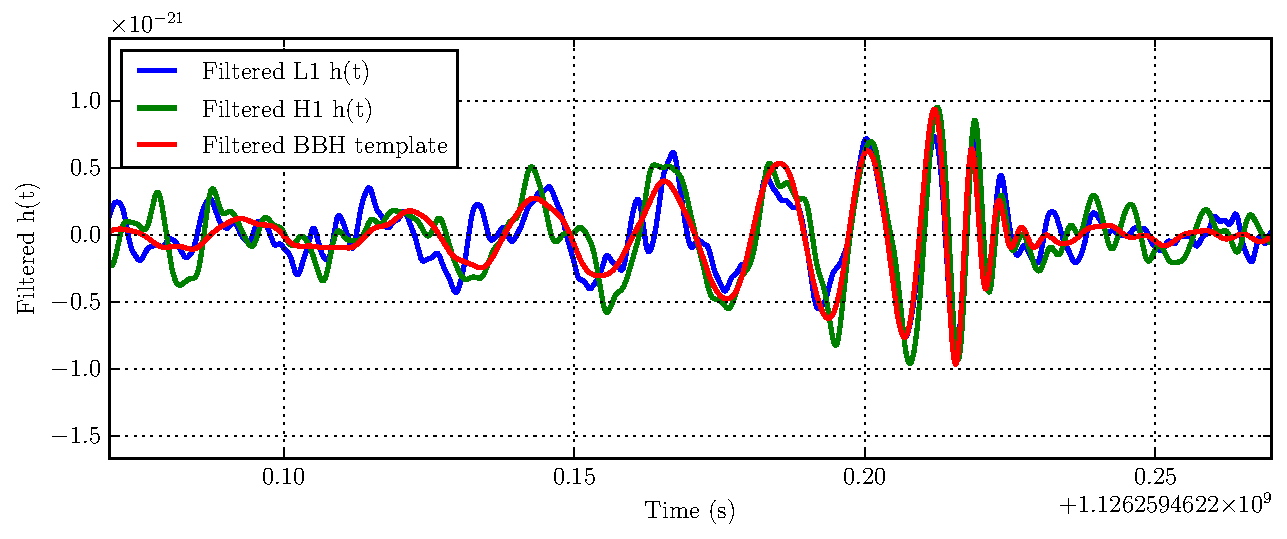
\includegraphics[width=\textwidth]{figures/O1/GW150914-timeseries}
\caption[GW150914 timeseries]{Time domain representation of H1 and L1 %
        gravitational wave strain at the time of GW150914. The blue %
        and green curves are detector strain, $h(t)$, zero-phase bandpass %
        filtered to isolate the %
        frequencies that contain signal. The red curve is a CBC waveform %
        generated using the best estimated parameters. The CBC waveform %
        has been filtered in the same way as the strain curve. The overlap %
        between the three curves is significant, demonstrating many cycles %
        of clear coherence and demonstrating the expected 'chirp' signal.}
\label{fig:GW150914}
\end{figure}

It is exceptional that GW150914 is visible in the detector data with 
such simple filtering. Due to the high total mass of the system, 
which is detailed in Table \ref{table:foreground}, the black holes 
of GW150914 coalesced quickly and at a low frequency, spending about 
0.2 seconds in the frequency range that aLIGO is sensitive to. The 
signal was also tremendously loud due to its high total mass and relatively 
close distance. 
As a result, the power in the signal is highly localized in time, 
producing a short, loud waveform that is readily visualized.
(A discussion of the data validation process relevant to GW150914 is 
found in Section \ref{sec:GW150914-validation}.)

\subsection{GW151226}

The other binary black hole signal discovered in O1, GW151226, has a rather different 
morphology. The system that produced GW151226 was roughly three times 
less massive than that of GW150914 and merged 
at a similar distance (see Table \ref{table:foreground}). Due to the 
lower total mass, GW151226 has an overall lower amplitude than GW150914 
and has its power distributed more broadly in time. GW151226 spent about 
2 seconds in the frequency band that LIGO is sensitive to, which is a 
factor of 10 longer than the duration of GW150914. For these reasons, 
it is not feasible to generate a time domain visualization of the signal. 
Thus, this is a dramatic demonstration of the value of a 
matched-filter search for CBC signals, which is designed to identify 
modeled signals buried in noise. 

\subsection{LVT151012}

The third loudest foreground event in the analysis, LVT151012, stands out 
from the background distribution but is not statistically significant 
enough to be labeled as a gravitational wave detection \cite{O1:BBH}. 
Its statistical 
significance is calculated to be just under $2\sigma$. While it is not 
being claimed as a gravitational wave detection, there is no obvious 
reason to believe that it is a noise artifact based on detector 
performance. It is possible that LVT151012 is part of a larger 
population of gravitational waves that is expected to contain 
quiet, threshold signals as well as clear detections.

\begin{table}[ht!]%
  \begin{center}
    \footnotesize
    \begin{tabular}{ccccccc}
    \hline
    Event & Time(UTC) & FAR ($\mathrm{yr}^{-1}$) & $m_1$ ($M_{\odot}$) & $m_2$ ($M_{\odot}$) & 
    $\chi_{eff}$ & $D_L$ (Mpc) \\
    \hline
    GW150914 & \begin{tabular}{@{}c@{}}14 September \\ 2015 \\ 09:50:45 \end{tabular} & 
    $< 5.8\times10^{-7}$ & $36_{-4}^{+5}$ & $29_{-4}^{+4}$ & $-0.06_{-0.18}^{+0.17}$ & 
    $410_{-180}^{+160}$ \\
    GW151226 & \begin{tabular}{@{}c@{}}26 December \\  2015 \\ 03:38:53 \end{tabular} & 
    $< 5.8\times10^{-7}$ & $14_{-3}^{+9}$ & $8_{-3}^{+2}$ & $0.20_{-0.10}^{+0.21}$ & 
    $490_{-210}^{+180}$ \\
    LVT151012 & \begin{tabular}{@{}c@{}}12 October \\ 2015 \\ 09:54:43 \end{tabular} & 
    0.44 & $23_{-5}^{+18}$ & $13_{-5}^{+4}$ & $0.0_{-0.2}^{+0.3}$ & 
    $1100_{-500}^{+500}$ \\
    \hline
    \end{tabular}
  \end{center}
  \caption[Table of foreground events]{Table of foreground events found in the first %
           observing run. %
           The quoted false alarm rates are calculated by the PyCBC search pipeline. %
           The GstLAL search pipeline reported similar results. %
           The astrophysical parameters are further explained in the parameter estimation %
           companion paper \cite{GW150914-PARAMESTIM}. % 
           Two binary black hole systems, GW150914 and GW151226, were %
           discovered with a false alarm rate $< 5.8\times10^{-7}$, which is the upper %
           limit on false alarm rate set by the amount of time used in the analysis. %
           This corresponds to a statistical significance $> 5.3\sigma$. %
           A third event, LVT151012, was an interesting foreground event that was not %
           statistically significant to be claimed as a detection, but could be part %
           of a larger gravitational wave population that includes weaker signals.
           } 
  \label{table:foreground}
\end{table}

\section{CBC Results}

The search for compact binary
coalescences was performed by two search pipelines: 
PyCBC \cite{pycbc-github,Usman:2015kfa} and 
GstLAL \cite{gstlal-methods}. 
In addition to these searches for modeled sources, an unmodeled 
burst search, Coherent Wave Burst (CWB), was run to search for coherent 
transient signals in the two Advanced LIGO interferometers \cite{GW150914-BURST}. 
All three of these analyses were able to recover GW150914. GW151226, 
having its power spread out over a longer period of time, requires a 
matched filter search and was not recovered by CWB. The two matched filter 
search produced consistent results. 
For brevity, we will focus on the results of the PyCBC search pipeline.

Figure \ref{fig:pycbc-hist-gw150914} shows the results of the PyCBC search 
over the whole of the first observing run \cite{GW151226}. The black curve shows the 
number of expected foreground events at a given $\hat{\rho_c}$ based on 
background noise for the analysis. For this curve, GW150914 is 
allowed to remain in the data when generating a background from timeslides. 
This answers an interesting question: if GW150914 is considered to be a 
chance coincidence due to noise, could a combination of GW150914 in 
one detector and background noise in the other detector generate a 
signal as loud is GW150914?

The blue curve shows the search background when GW150914 is removed 
from the analysis and not used when generating a background from 
timeslides. Since we believe that GW150914 is a real gravitational wave 
signal, using it in background calculations no longer provides a 
search background that is a realization of detector noise alone 
when evaluating the significance of quieter signals. 
If GW150914 is allowed to produce background events, the 
significance of GW151226, which is represented by the orange square at 
$\hat{\rho_c} = 12.6$, is highly diminished. This can be seen by comparing 
the blue and black curves. The differences between them, including the 
extension of the background to $\hat{\rho_c} = 21$ , are the result 
of GW150914 combining with background noise.

The orange squares indicate the 
number of foreground events that were actually recovered by the search 
pipeline. 
The statistical significance of a given foreground event is 
the determined by the rate at which detector noise produces background 
events with a detection statistic higher than that of the signal 
\cite{GW150914-CBC}. The false alarm rate for a given foreground 
event is defined as the rate of background events with a $\hat{\rho_c}$ 
greater than or equal to that of the foreground event. This rate 
can be converted into a false alarm probability by assuming that the 
background events follow a Poisson distribution. 

GW150914 
was an exceptionally loud signal and is the loudest event in the 
analysis. Since there are no background events as loud as GW150914, 
its statistical significance has a lower limit of $5.3\sigma$ 
but is not exactly calculated. The associated statistical significance 
is listed on the horizontal bars on the top of the plot. The color 
of each bar corresponds to the background from which the statistical 
significance was measured.  

\begin{figure}[ht!]%
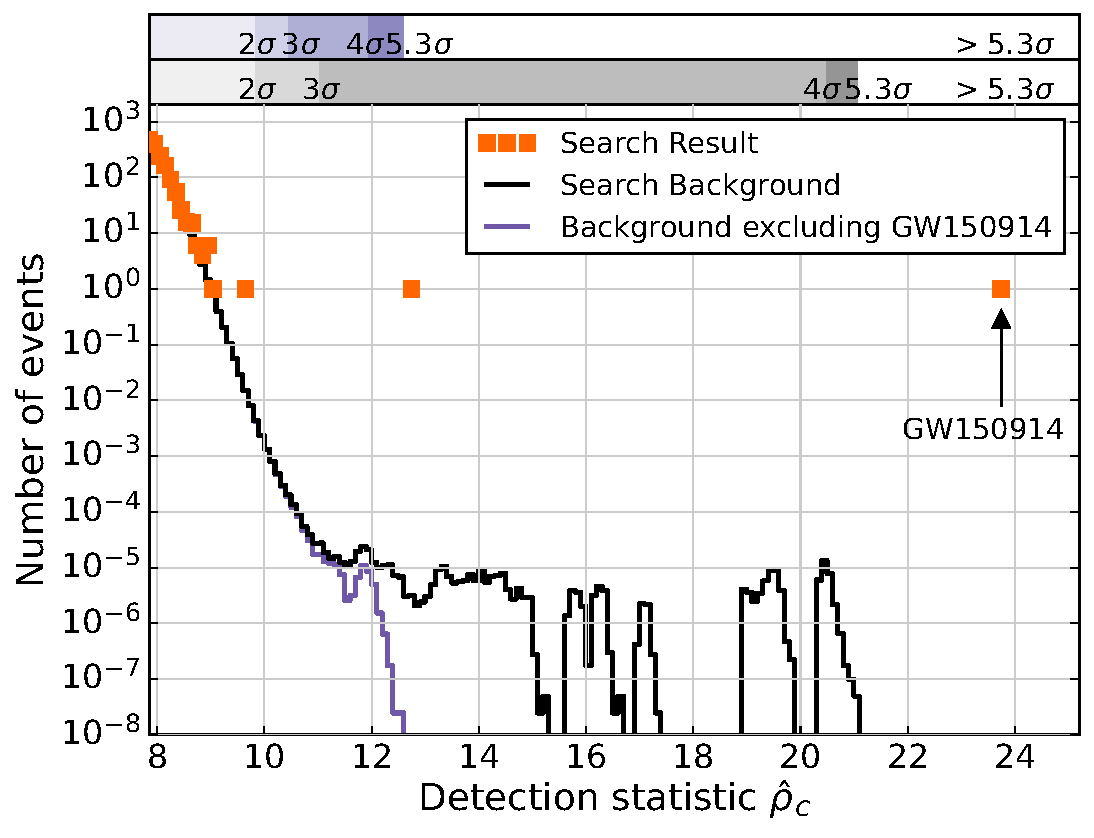
\includegraphics[width=0.85\textwidth]{figures/O1/pycbc_hist_GW150914}
\caption[PyCBC result histograms for GW150914]{PyCBC search results for %
         the first observing run. The black curve is the search background %
         relevant to GW150914. The blue curve is the search background %
         relevant to GW151226 where GW150914 has not been included in the %
         search background calculation. GW150914 was the loudest event in %
         the first observing run and was reported with a significance %
         $> 5.3\sigma$. Figure \ref{fig:pycbc-hist-gw151226} provides % 
         a better visualization of the significance of GW151226.}
\label{fig:pycbc-hist-gw150914}
\end{figure}

With GW150914 removed from the search background, we can correctly evaluate the 
statistical significance of GW151226. 
Figure \ref{fig:pycbc-hist-gw151226} shows a zoomed in version
of the search background with GW150914 removed. 
GW151226 is the loudest event in the analysis once GW150914 and its associated 
background triggers have been removed. Since there are no background events 
as loud as GW151226, its false alarm rate can be bounded to 1 per the entire 
analysis time. The associated statistical significance has a lower limit of 
$5.3\sigma$ but can not be directly calculated. The blue curve in this plot 
shows the search background with GW151226 removed from the analysis. Any 
quieter foreground triggers, such as LVT151012, will have their false alarm 
rate and statistical significance determined by this background distribution.  
LVT151012, which is the second loudest foreground event in Figure 
\ref{fig:pycbc-hist-gw151226}, was recovered at $\hat{\rho_c} = 9.6$ and 
assigned a statistical significance of just under $2\sigma$ as it was 
not louder than all background events.  Since there are many background 
events that are louder than LVT151012, there is no significant change 
in the background distribution if LVT151012 is removed before performing 
time slides to generate the background. 

\begin{figure}[ht!]%
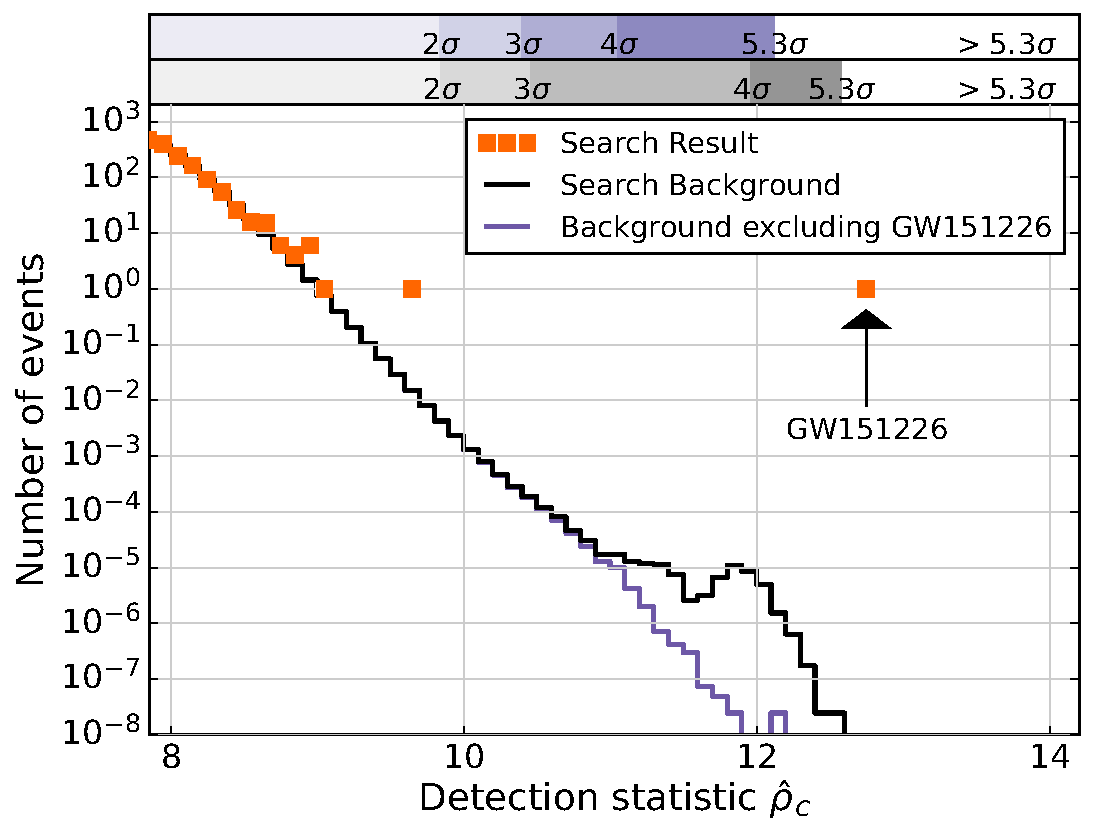
\includegraphics[width=0.85\textwidth]{figures/O1/pycbc_hist_GW151226}
\caption[PyCBC result histograms for GW151226]{PyCBC search results for the %
         first observing run with GW150914 removed. The black curve is the %
         complete search background. The blue curve is the search background %
         when GW151226 is removed and not allowed to combine with noise to %
         generate background events. In both cases, GW151226 is the loudest %
         event in the analysis. The statistical significance of GW151226 %
         is bounded to be $> 5.3\sigma$. The second loudest event in this %
         plot is LVT151012, which is assigned a statistical significance of %
         just under $2\sigma$.}
\label{fig:pycbc-hist-gw151226}
\end{figure}

\section{Summary}

The search results of the first observing run are summarized in Table 
\ref{table:foreground}. False alarm rates are quoted as estimated by the 
PyCBC search pipeline.  
The two discovered binary black hole signals, GW150914 and GW151226, differed 
by about a factor of 3 in total mass and originated at similar distances 
from Earth, which is responsible for the higher SNR  
of GW150914. Both events are estimated to have occurred at similar distances, 
with their error regions having significant overlap. 
The third interesting foreground event,
LVT151012, is estimated to have a total mass greater than GW151226, but its
distance is estimated to be much further away.

The estimated distance for 
GW150914, 410 Mpc, corresponds to 1.3 billion light years. Since general 
relativity predicts that gravitational waves travel at the speed of light, 
this means that the signal we measured as GW150914 was emitted 1.3 billion 
years ago, before complex life existed on Earth. For reference, 
the Andromeda Galaxy is less than 1 Mpc away from Earth. 

Both GW150914 and GW151226 were the loudest events when compared to their 
respective background distributions, resulting in a false alarm rate 
$< 5.8\times10^{-7} \mathrm{yr}^{-1}$, which corresponds to a statistical significance of 
$> 5.3\sigma$. LVT151012 has a false alarm rate of $0.44 \mathrm{yr}^{-1}$, which 
corresponds to a statistical significance of just under $2\sigma$.

